\chapter{Introduction} \label{johdanto}


A Linux distribution is a bundle of the Linux kernel and a set of software products called packages \cite{gnuPackagesx2014}. A package manager is an instrument that handles building packages from either from source or pre-built binaries, resolving build-time and run-time dependencies of packages and installing, removing, and upgrading packages in user environments \cite{gnuPackagesx2014}. Every Linux device must handle its installed programs with their dependencies and configurations either imperatively or declaratively. Overwhelmingly large portion of Linux distributions fall in to the first category \cite{dolstra2008nixos}. Both imperative and declarative systems have their strengths and weaknesses from administrative and security standpoints.

An imperative system provides updatability and modification through a destructive instrument. Popular imperative package managers are apt, apk, dnf and zypper \cite{dolstra2008nixos}. Imperative package managers can remove and overwrite existing files which leaves the system in an inconsistent state. Different installs have by nature different states which causes many problems discussed in this thesis. Mainstream distributions such as Debian or Fedora, which are depicted in figure \ref{timeline}, base a huge portion of their functionalities on an imperative package manager.

As files are cross-modified through packages with package managers such as apt, upgrading can be disastrous and such systems don't support atomic rollback capabilities \footnote{Some Linux distributions using btrfs filesystem can perform a snapshot and rollback\cite{opensuseSystemRecovery}}. Due to the unpredictability, often the result can be a partially or completely broken system. \cite{dolstra2008nixos}

The reference imperative system in this thesis is Debian with it's default package manager apt due to it's popularity and relative simplicity. The reference declarative system on the other hand is NixOS with it's partial namesake package manager Nix. NixOS is a Linux distribution that is based on Nix and provides declarative configuration of the whole system including the Linux kernel\footnote{There exists an experimental project that has succeeded with BSD interoperability}. Nix is configured by the Nix programming language which is inspired by purely functional languages such as Haskell. The Nix programming language is referred as Nix language in this thesis. \cite{van2013reference}

The reference architecture depicted in chapter \ref{architecture} is based on NixOS as it is the most popular purely functional, declarative Linux distribution with over 100 000 packages \cite{nixosNixOSSearch}. Another good alternative would have been Guix, which has over 28 000 packages \cite{gnuPackagesx2014}. Guix has some improvements over Nix, including richer and more extensible programming environment with a Lisp-dialect configuration language, Scheme \cite{courtes2021deploiements}. NixOS remains as the distribution of choice, as the number of packages is greater, and general support is found to be better.

This thesis focuses on the systems and information security of a reference architecture created with NixOS. Chapter \ref{architecture} goes through a whole reference architecture of a solution that handles securely the most critical functionalities of a reference embedded server and fleet.
\begin{figure}
    \centering
    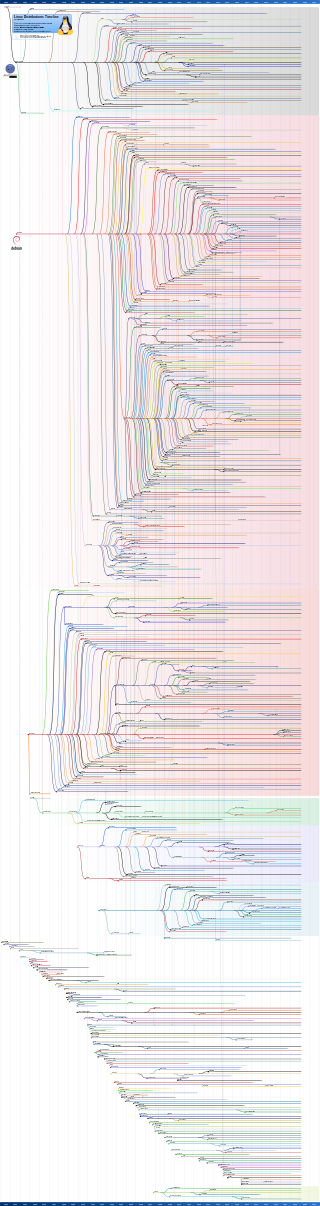
\includegraphics[scale=0.4]{latex/kuvat/timeline.png}
    \caption{Distribution of Linux distributions. From top left to bottom: Slackware, Debian, Red Hat, Jurix and smaller distributions, including NixOS (https://en.wikipedia.org/wiki/List\_of\_Linux\_distributions#/media/File:Linux\_Distribution\_Timeline.svg)}
    \label{timeline}
\end{figure}

This thesis discusses how declarative systems can be used as an improvement over imperative systems. In chapter \ref{imperative} both approaches to package management is compared, and in chapters \ref{architecture} and \ref{analysis} a quantitative research is carried out revealing strengths and weaknesses of the reference Nix environment setup. Selected methodologies provide quantitative results which can be used to improve the security of similar declarative systems. Propositions for further research are gone through in chapter \ref{further} and finally, chapter \ref{conclusion} concludes the thesis.

\section{Research methodologies and questions}

Research methodologies used in this thesis are:
\begin{enumerate}
\item a literature review of central papers on subject themes found with prepared search statements
\item an action research using a laboratory setup
\item a quantitative research process
\end{enumerate}

Literature review will be addressed in the next section. As this thesis' main research methodology is quantitative, the gathered data points will be addressed as variables that are compared with mathematical methods. Quantitative methods are broken down in chapter \ref{securitystandpoints} and \ref{analysis}. The central methodology is derived from QuERIES, and the information security aspect is investigated with CIA-triad. In chapter \ref{analysis} section \ref{whyqueries} QuERIES is compared with other metrics which are explained in subsection \ref{resquest}.

Quantitative methodologies are oftentimes used in conjunction with qualitative methodologies, both approaches having their strengths and weaknesses. One drawback of using qualitative methods in security framework is their inherent subjectivity. For example the Delphi technique, where a set of opinions is gathered and compared from a working group provides subjective substance for a study instead of objective perspectives \cite{wang2005information}.

The study design in this thesis is \textit{state based}, which refers to the fact that the research methods focus on different state transitions, e.g how probable it's for an intruder to gain from partial leverage to a full control of a system. Qualitative research wouldn't alone satisfy the requirements, as investigating different state transitions without quantitative methodologies would be absurd \cite{ramos2017model}.

\subsection{Literature review}\label{litrev}

This thesis has bibliography from x sources, most of it gathered with a carefully prepared search statement. Other sources include manuals, material for research methods and other relevant material. The search statement's results, presented in next subsection, provide good base for action research and analysis.

The literature focuses on three main concepts: embedded systems security with and without declarative components, imperative systems and NixOS as a solution. The main goal is to find literature that combines these concepts to gain platform for comparing different approaches to support the action research. 

Central literature revolves around Nix and multiple texts by Eelco Dostra are cited for illustrating the nuances of a Nix ecosystem. Other declarative approaches are discussed, i.e by Endres et. al and Van der Burg \cite{van2010declarative, endres2017declarative}. These approaches also contains comparison to imperative systems, which is the central approach in chapter \ref{imperative}. Combining cyber security with declarative approaches were discussed by Specht et. al and Kandoi and Artke \cite{specht2007analysis, kandoi2021operating}.

Material discussing embedded security and security standpoints in general are adequately discussed by Ravi et. al and Fysarakis et. al \cite{ravi2004security, fysarakis2014embedded}. The concepts, however are generally too broad for this thesis' scope, so only the most fitting approaches were selected for use.


\subsubsection{Search statement} \label{s-}

The main search statement for this thesis is:
"embedded linux" OR ''declarative'' AND (linux OR *nix) OR deployment OR ''system update'' OR (compare* AND declarative AND imperative AND system*) OR security.

The search statement was prepared to provide as relevant results as possible for this thesis. The main goal was to include the hypernyms ''embedded linux'', ''linux'' witch other terms separated using the "OR" operator. The subterm (compare* AND declarative AND imperative AND system*) was chosen to broaden the search to include articles which compare declarative and interactive systems.

As security is a central theme in this thesis, the term "security" was included. Search was done on Google Scholar, and other useful material was handpicked, such as NixOS manuals and wiki pages. Systems security and cyber security material is also included in the bibliography using search statement systems security OR cyber security. Separate search ''cia-triad'' and ''partial observable Markov chain'' AND ''cybersecurity'' were used to provide more tangible meters for measuring cyber security. To further back up the research for comparing different metrics, term ''cyber security metric methodology'' was searched.

For searching specific material about embedded systems, the search statement ''embedded AND security'' was used. As the need for embedded toolchains was needed, statement ''yocto AND buildroot'' was searched. All searches were done on Google Scholar platform.


\subsection{Research questions} \label{resquest}

The research questions for this thesis are:

\begin{enumerate}
\item How can a declarative system be used to improve the basic security needs of an embedded system used for displaying public media measurably?
\item What are the advantages and/or disadvantages of such system from system administrator standpoint?
\item How can a declarative system be updated from different Linux distribution securely and seamlessly?
\end{enumerate}

Research question 1 is perhaps the most important and it traverses through themes of the whole thesis. The hypothesis is that traditional imperative embedded device fleets have problems that can be solved with the use of modern declarative systems. First, we aim to gain information from a specific scenario, presented in chapter \ref{architecture}, then in chapter \ref{analysis} the gained information is analyzed and generalized as suitably as possible. 

Research question 2 brings up the human element; how can a system administrator use a new palette of features adequately to provide more secure system and research question 3 handles a situation where existing framework should be replaced with a NixOS system. How this could be done securely, without risks and preferably easily with existing or new tooling, is answered in chapter \ref{architecture} section \ref{instnewdevices}.

\subsection{Data collection and analysis}

Data collection is done with simulated red–blue team setup, where either team has a time frame where they must conduct a series of tasks. These tasks are formalized as partially observable Markov chain parameters, and analysed with QuERIES methodology. This methodology is used to gain knowledge and make the system more reliant and better. Chapter \ref{analysis} answers research questions quantitatively and provides analysis for the reference system.
















